%
\chapter{Introduction}\label{chap:introduction}%
%
    \textit{%
        In light of the depletion of conventional, natural and fossil fuels for energy production, as well as their negative impact of their consumption on the environment, renewable, clean - virtually emissionless - and readily available alternatives are direly called for. Despite its, for now more than 70 years persisting technical and economical challenges, magnetically confined plasma nuclear fusion is a prime candidate for such and has the potential to be the final answer to issues of ongoing climate change, the associated accelerated growth in energy consumption, costs and the discrepancy of global resource distribution\cite{IPCC2023,Toschi1971}.
    }%
%
    \section{Nuclear Fusion}\label{sec:section}%
%
        Nuclear fusion is the process of two lighter atoms or nuclei interacting and forming a heavier element. This phenomenon has been thoroughly studied since its discovery in the early 20th century on our solar systems central star \textit{sol}\cite{Oliphant1934}. Ironically, initial research around nuclear fusion was based on weapons development surrounding the \textit{Manhattan project}\footnote[1]{a program of research and development during WWII to produce nuclear weapons, led by the United States in collaboration with the United Kingdom, resulting in two bombs dropped on Japan} \textit{thermonuclear bombs} and later iterated upon by scientist in the United Kingdom and finally brought to a first concept individually in 1950/51 by Lyman Spitzer\footnote[2]{Lyman Spitzer, Jr. *\,Jun. 26, 1914 Toledo; \textdagger\,Mar. 31, 1997 Princeton} in the USA, as well as Andrei Sacharow\footnote[3]{Andréj Dmítrievič Sácharov, *\,May 21, 1921 Moscow; \textdagger\,Dec. 14, 1989} and Igor Tamm\footnote[4]{Igor' Evgen'evič Tamm, *\,Jun. 26, 1895 Wladiwostok; \textdagger\, Apr. 12, 1971 Moscow} in the USSR. All postulated magnetic plasma confinement as way to a thermonuclear reactor, however with different approaches, i.e. the \textit{stellarator} and \textit{tokamak}. Since then, nuclear fusion has been experimentally demonstrated in laboratory environments and hence associated with the fourth state of matter, \textit{plasma}\cite{Shafranov2001}.\\%
        Fusion processes involving light nuclei, i.e. hydrogen or helium isotopes are energetically most advantageous, as they produce the most energy per nucleus mass. In the case of confined, high-temperature plasma applications, such large kinetic energies and therefore velocities are necessary to overcome the electrostatic Coulomb force repulsion between the positively charged nuclei, reducing the distance so that the \textit{strong nuclear force} dominates and fusion reactions are induced. Rate coefficients $\left\langle\sigma v\right\rangle$ towards the total yield $Q=P\ix{fus}/P\ix{ext}$, with $P\ix{fus}$ the power from fusion reactions and $P\ix{ext}$ the input, are convolutions of kinematic cross-sections and Maxwell-Boltzmann distributions. Of those, only a Deuterium-Tritium interaction has a large enough contribution at energies $\le$\SI{64}{\kilo\electronvolt} due to an intermittent resonance in a volatile $^{5}_{2}$He\cite{Bosch1992}.
%
            \begin{align}%
                ^{2}_{1}\text{D}+\,^{3}_{1}\text{T}\longrightarrow\,^{5}_{2}\text{He}^{\ast}\longrightarrow\,^{4}_{2}\text{He}\left(\text{\SI{3.5}{\mega\electronvolt}}\right)+\,^{1}_{0}n\left(\text{\SI{14.1}{\mega\electronvolt}}\right)\label{eq:dtfus}%
            \end{align}%
%
        Resulting kinetic energies of the products are noted accordingly. Plasma temperatures of \SI{20}{\kilo\electronvolt} have been achieved regularly and by a large range of devices, underlining the superiority of DT fusion in this regard. The vast energy gain on the right-hand-side in \cref{eq:dtfus}, particularly the fast neutrons can be used to heat a water repository in a future power plant, similar to a conventional nuclear fission reactor. Additionally, only minor secondary radioactive waste from neutron activation is expected from such a device, alleviating the issue of dismantlement and final storage of other nuclear machines. Deuterium has a sufficient natural abundance and hence can be distilled effectively from water, while Tritium does not but can be \textit{bred} using the penetrating neutrons and a supplementary Lithium blanket around the vessel.\\%
%
        \newline%
        This thesis is concerned with the properties of radiation in the stellarator \textit{Wendelstein-7X} (W7-X), particularly from intrinsic and extrinsic impurities, their transport and effects on the overall plasma performance. After an introduction to the machine, presented results will be centred around the core diagnostic responsible for measuring radiation at W7-X: the \textit{multicamera, metal resistor bolometer}. The next sections will introduce the core concepts relating to the investigations performed in this work.%
%
    \section{Wendelstein 7-X}\label{sec:w7x}%
%
        \begin{figure}%
            \centering%
            \includegraphics[width=0.5\textwidth]{%
                content/figures/chapter0/w7x}%
            \caption{Stellarator Wendelstein 7-X: Cut-away rendering of the outer vessel, superconducting magnetic coils, cooling and supporting structure. The translucent red band is the plasma tube (last closed magnetic flux surfaces). \textcopyright IPP}\label{fig:w7x}%
        \end{figure}%
%
        Wendelstein 7-X is the latest iteration in a long line of stellarator experiments conducted by scientists at the Max-Planck Institute for Plasma Physics, beginning in the 1950s. The first W1-A stellarator went into operation in 1960 at the Max-Planck Institute for Physics and Astrophysics, providing a foundation for the continuing development of which this device is the culmination.\\%
        Stellarators generate the necessary rotational transform, the twist of the magnetic field, (majorly) by external coils. Consequently, the stellarator magnetic field is deliberately configured using said coils and its plasma essentially current-less and more stable compared to a tokamak. Wendelstein 7-X is designed to be modular, i.e. have a discrete symmetry that enables entire subsections to be replaced or exchanged. The iterative optimisation process towards such a modular device was shaped to satisfy multiple criteria, including small magnetic islands, good plasma equilibrium and magnetohydrodynamic (MHD) stability, reduced neoclassical transport, minimized bootstrap current and fast particle confinement. Its modular designed, five-fold symmetric superconducting magnetic field coils encompass the whole machine. The coil system consists of 70 superconducting magnets of seven different shapes, 50 non-planar coils producing the twisted magnetic field and 20 planar coils for increased flexibility in magnetic configuration space - it can be seen in \cref{fig:w7x}\cite{Spitzer1958,Boozer1998,Wagner1998,Beidler1990}.\\%
        The W7-X stellarator is the largest of its kind, with a major and minor radius of \SI{5.5}{\meter} and \SI{0.53}{\meter} (depending on magnetic coil currents) respectively, volume of \SI{30}{\cubic\meter}, \SI{3}{\tesla} maximum magnetic field strength, heating power of \SI{14}{\mega\watt} and expected plasma temperatures of up to \SI{130}{\mega\kelvin}. W7-X has performed three successful experimental campaigns since its first plasma in 2015. After multiple upgrades, the machine has demonstrated improved, longer confinement and increased overall power, with the ultimate goal being a discharge duration of \SI{30}{\minute} at \SI{10}{\mega\watt} of external heating, demonstrating a capability essential to a future fusion power plant: continuous operation\cite{Klinger2016_2}.\\%
        Development of this stellarator reactor line was defined by the qualification of a viable divertor concept. Divertors - interfaces deliberately contacting and \textit{diverting} (interacting) with the hot plasma - in stellarators cannot be toroidally symmetric. The cross-section of W7-X varies strongly from triangular to bean-shape and exhibits natural magnetic islands, i.e. smaller, from the core separated and confined flux tubes which do not extend far toroidally. Hence, so-called \textit{island divertors} are placed at the edge where the rotational transform has a resonance close to unity. This field line pitch $\iota$ is defined as the number of poloidal transits per single toroidal transit of a field line on a toroidal flux surface. Assuming toroidally nested magnetic flux surfaces, the rotational transform is given by $\iota/2\pi=\diff\psi/\diff\Phi$, with $\psi$ the poloidal magnetic flux, and $\Phi$ the toroidal magnetic flux. The tube of the last closed flux surface (LCFS) and cuts through the magnetic field structure for characteristic points can be found in \cref{fig:trianglebeanFS}. On each magnetic field period, one pair of island divertor modules is installed where the cross-section of the magnetic field is predominately bean-shaped. Magnetic islands intersect these targets, providing a well-defined flow of particles from the plasma \textit{scrape-off layer} (SOL) to the wall and decoupling the core plasma region in the process. Divertors therefore have to withstand a heat flux of up to \SI{10}{\mega\watt\per\square\meter}. Wendelstein 7-X was not yet equipped with water-cooling and plasma contact points are only inertially cooled in experiments discussed for this thesis\cite{Geiger2015,Beidler1990}.%
%
        \begin{figure}%
            \centering%
            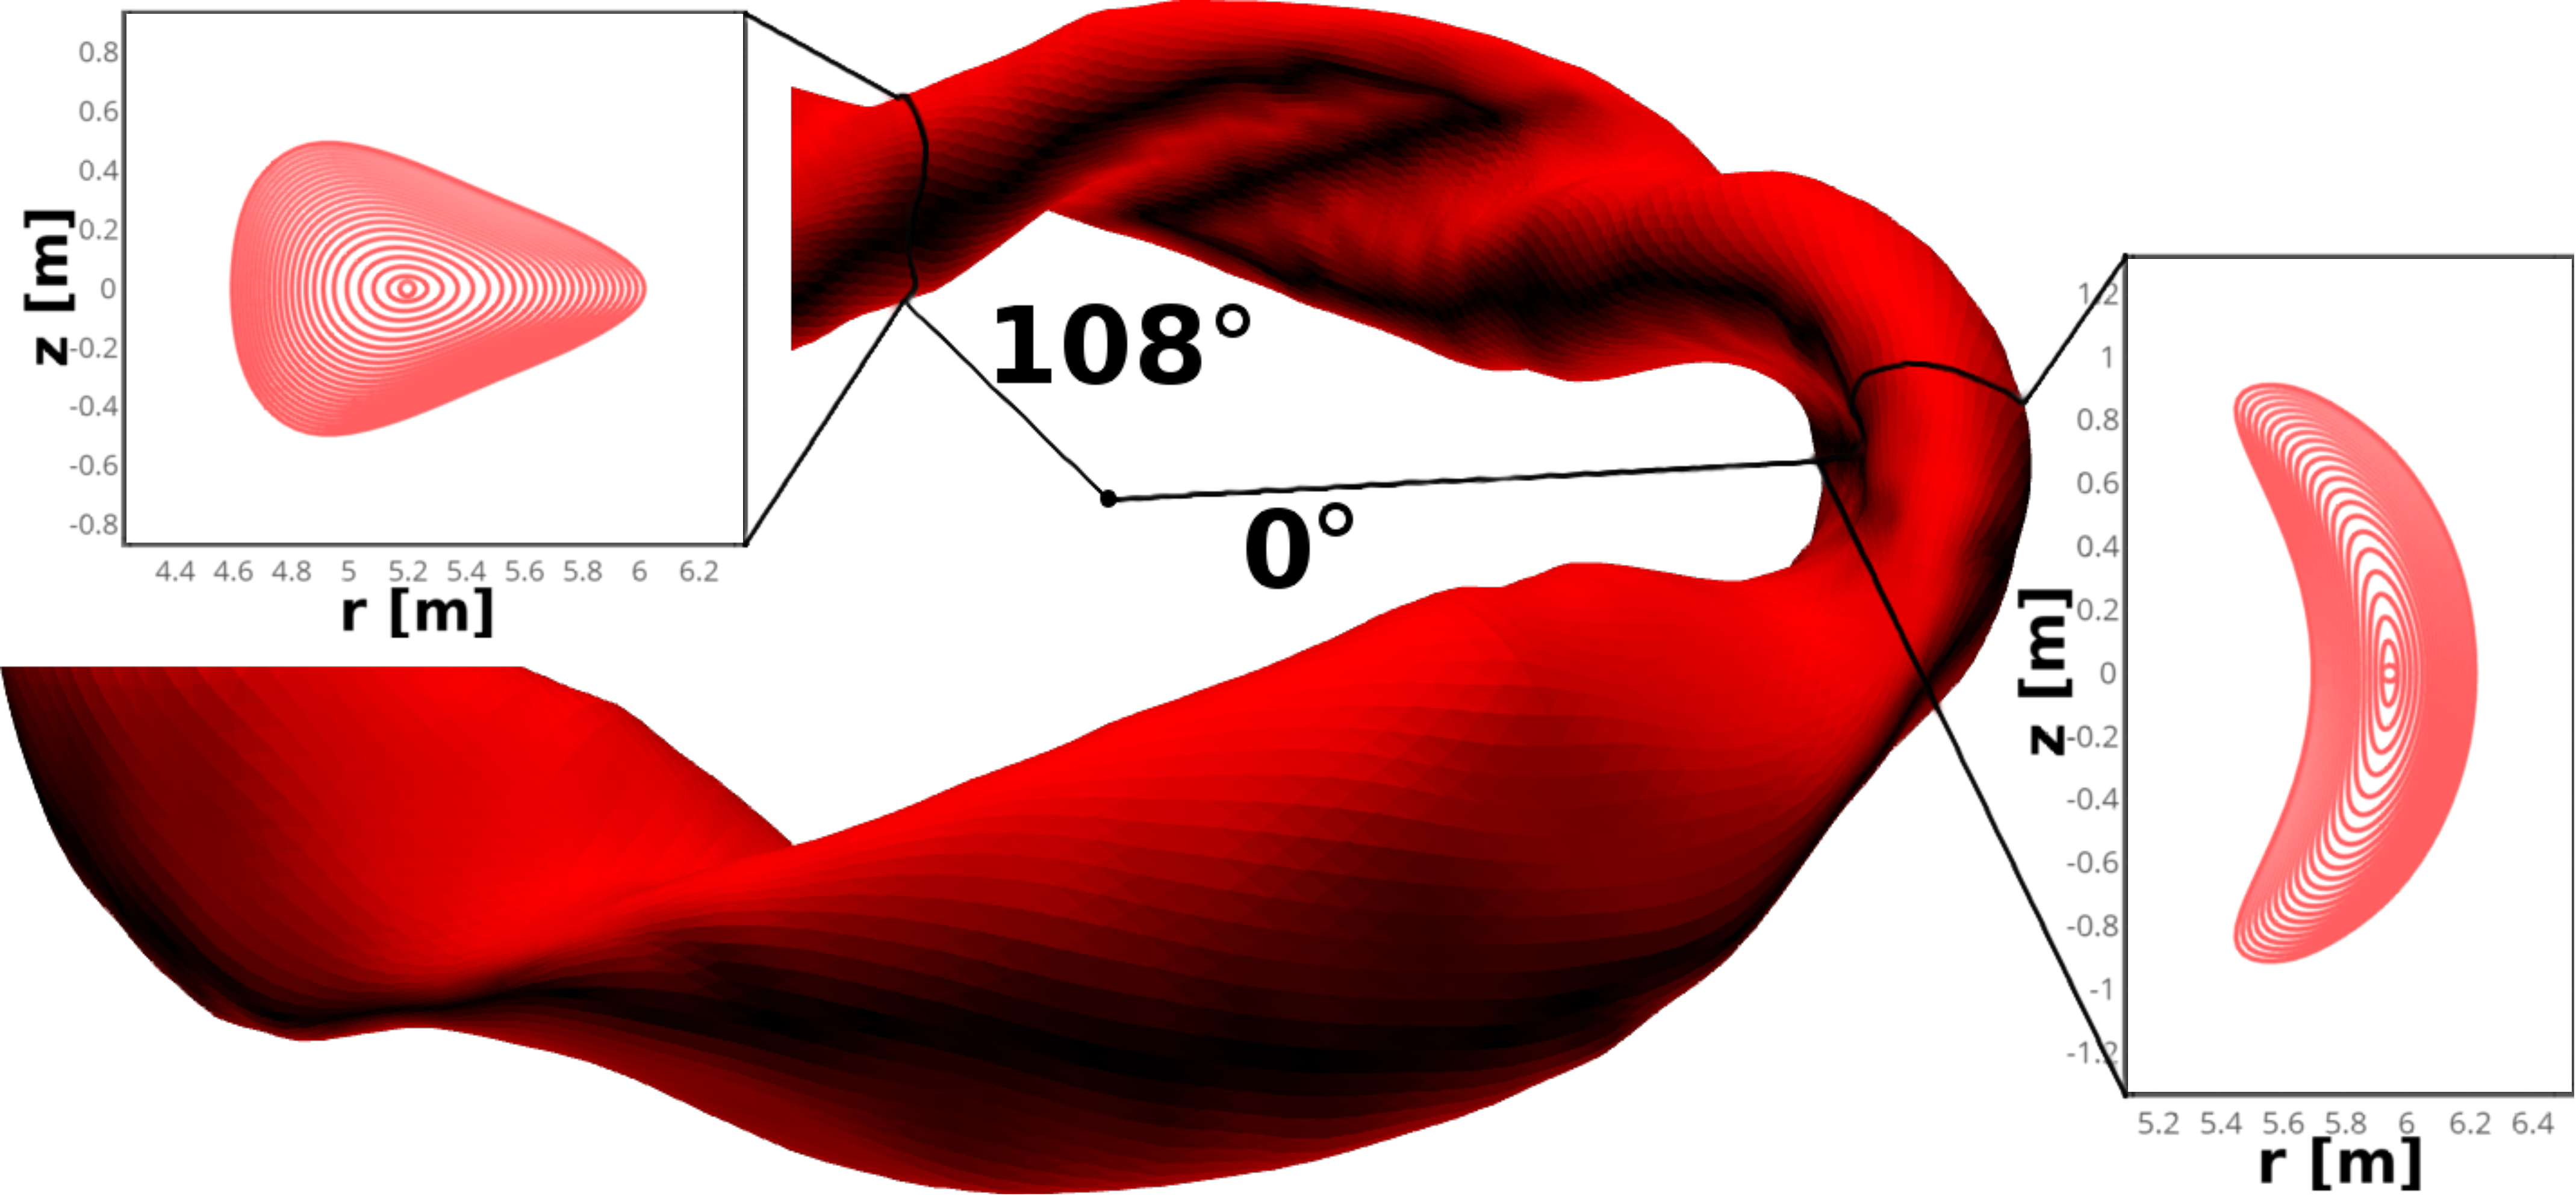
\includegraphics[width=0.6\textwidth]{%
                content/figures/chapter0/torus_full_banana_alpha.png}%
            \caption{Flux tube of the last closed flux surface around the W7-X torus and cross-sections in the triangle- (left) and bean-shaped (right)plane. At \SI{108}{\degree} toroidally, the bolometer camera system is located.}\label{fig:trianglebeanFS}%
        \end{figure}%
%
    \section{Plasma Physics}\label{sec:plasmaphysics}%
%
        At the given temperatures, matter only exists as plasma, an ionized gas where atoms are fully ionized and interact with electric and magnetic fields. Hence, fusion energy research is the study of high-temperature plasma physics in large devices with strong magnets. Challenges here are the long-time confinement of particles and exhaust of thermal energy, while a lower limit for a self-sustaining or -heating fusion plasma $Q>1$ is given by the \textit{triple product} or \textit{Lawson criterion}. Introduction of non-hydrogenic species into the plasma via deliberate gas puffing, solid-state seeding, sputtering of wall material or intrinsic impurities has to be taking into account due to its parasitic and diluting effect on the system:%
%
        \begin{align}%
            n\ix{e}\tau\ix{E}\ge\frac{12f\ix{tot}}{\left\langle\sigma\ix{DT}v\right\rangle f\ix{H}^{2}E_{\alpha}-4L\ix{Z}\left(T\right)}\,T\,\,\label{eq:lawson}%
        \end{align}%
%
        with $n\ix{x}$ the number densities and $T$ the equilibrated temperatures of electrons, ions and atomic hydrogen respectively, $f\ix{H}=n\ix{H}/n\ix{e}$ the hydrogens fractional abundance, $f\ix{tot}=\sum_{i}n\ix{i}/n\ix{e}$ the ion-electron dilution, $E_{\alpha}$ kinetic alpha particle energy and $L\ix{Z}$ the radiative loss function. Plasma conditions described by satisfying the Lawson criterion in \cref{eq:lawson} require a strong magnetic confinement, trapping charged particles in the magnetic field using
        the Lorentz force to restrict their motion perpendicular to its field and travelling in a \textit{gyro-motion} on helical trajectories along those lines. In stellarators, additional drift effects are compensated by the secondary poloidal magnetic field from the sophisticated magnetic coil setup\cite{Helander2014,Boozer2015}.\\%
        In current and future plasma fusion devices, large heat loads on plasma facing components are a challenge and topics surrounding it of great scientific interest, as steady-state operation at large powers is central to the ultimate goal of a nuclear fusion power plant. The expected huge power flux onto divertors for such a scenario of continuous operation are significantly larger than the material limits. Distribution of this energy and thermal load through electromagnetic radiation into the full $4\pi$ solid angle and onto the entire vessel wall is one possible solution to this problem. \textit{Bremsstrahlung} $P\ix{brems}$ of accelerating charged particles on field lines and line radiation from ionisation and excitation processes $P\ix{line}$ contribute to the \textit{cooling} of the core. Steady-state, the plasma confinement power balance can be written as $P_{\alpha}+P\ix{h}=P\ix{n}+P\ix{rad}^{\text{core}}+P\ix{SOL}$, with $P_{\alpha}$ the alpha particle \textit{heating} of the plasma, $P\ix{h}$ the external input, $P\ix{SOL}$ the total power in the SOL and $P\ix{rad}^{\text{core}}=P\ix{brems}+P\ix{line}$. Introduction or seeding of extrinsic, high-Z impurities into the core, which radiate strongest in the hotter confinement center can be used to increase the latter and hence reduce the power that enters the SOL\cite{Shubov2021,Schneider2006,Drawin1978}. The impact of deliberate plasma pollution however has drawbacks. Dilution is increased because of their greater number of charge states and are likely to accumulate in the core due to transport dynamics. Furthermore, oversaturation with impurities can lead to plasma termination, radiative collapses or disruptions. Varying operational and machine conditions, as well as impurity combinations inside the plasma and their different behaviour under those circumstances make the experimental evaluation particularly difficult\cite{Reimold2015}. This topic is center of ongoing investigations and ultimately motivation for the methodology and application developed over the course of this thesis. In the hypothetical first plasma fusion power plant prototype DEMO, it is expected that $0.7P\ix{h}$ is radiatively exhausted from the core and the remainder has to be further reduced through radiation in the SOL, finding at least a radiation fraction $f\ix{rad}=P\ix{rad}/P\ix{h}>0.95$. \textit{Radiation in the divertor} has several benefits, like a reduced total heat flux onto and broadening of the contact area with the target, decreasing chemical and physical sputtering of wall material and additional reaction loss channels with neutral particles. At the lower densities and temperatures outside the LCFS, low-Z impurities can be used to control the radiation here such that fuel dilution, impurity retention and radiative saturation of the divertor are of adequate levels\cite{Eich2013,Eich2011,Fuchert2020}.%
%
        \subsection{Transport}\label{subsec:tranport}%
%
            Transport plays a very important role in the performance of fusion devices. They transfer energy, mass and charge spatially via collisions between particles or by flows, thermodynamically equilibrating the plasma. Commonly, plasma transport refers to the combination of classical, neoclassical and anomalous or turbulent processes. Turbulent transport dissipates energy through non-linear, chaotic flows, which are themselves usually generated by instabilities in the plasma, and is very effective in transporting energy and mass.%
%
            \subsubsection*{Classical Transport}%
%
                Classical transport considers diffusive collisions between ions, eventually leading to a net particle loss from the confinement to the SOL and vessel walls. Due to the presence of charged particles, plasma diffusion significantly differs from diffusion in gases or liquids. The interaction between the positive and negative particles results in ambipolar diffusion with a diffusion coefficient that is dissimilar to that of either electron or ion species separately. The rate of diffusion scales with $1/B^{2}$, implying that confinement times can be greatly improved with small increases in field strength. Such collisions change the center of the particles gyrating motion, with displacements the size the Larmor radius $r\ix{L}$. Same species Coulomb collisions yield no net transport but may contribute to energy transfer and heat flux. With impurities, friction effects between all species need to be taken into account. Ion-impurity collisions dominate the impurity transport due the large collision frequency $\nu$, causing convection. The impurities diamagnetic velocity $v\ix{dia}$ is directed into the same direction as the diamagnetic velocity of the hydrogen ions. However, due to the charge dependence of $v\ix{dia}$ there exists a velocity difference between ions and impurities. The resulting friction force is amplified by the respective ion charge of the impurities. Due to the electrostatic repulsion, this translates into an inward convection of impurities and an outward convection of hydrogen. Radial temperature gradients however may change the convection proportionality due to the decrease in friction at larger relative velocities. Fluid models find an extra term $\propto\nabla T$ related to Coulomb friction, ultimately causing an outward flux of impurities. For an impurity of charge $q$, the total flux $\vec{\Gamma}\ix{q}$ including diffusive and convective transport can be written as%

                \begin{align}%
                    \vec{\Gamma}\ix{q}=\frac{r\ix{L,q}^{2}\nu\ix{q,H}}{2}\left(-\nabla n\ix{q}+n\ix{q}q\left(\frac{\nabla n}{n}-\frac{\nabla T}{2T}\right)\right)\,\,.\nonumber%
                \end{align}%
%
            \subsubsection*{Neoclassical Transport}%
%
                In practice, the rates suggested by classical diffusion have not been found in real-world machines, where a host of previously unknown plasma instabilities caused the particles to leave confinement at rates closer to $B$, as had been seen in Bohm diffusion. The failure of classical diffusion to predict real-world plasma behaviour led to a deeper understanding of the diffusion process, known as neoclassical transport.\\%
                The \textit{neoclassical transport model} provides a model for the transport of particles, momentum, and heat due to Coulomb collisions in confined plasmas in complex magnetic geometries, assuming that the plasma is in an equilibrated state, i.e. not including fluctuations. The classical model is extended by the incorporation of geometrical effects, which lead to complex particle orbits and drifts that were ignored in the latter.\\
                Writing the Boltzmann equation with the particle distribution function $f\ix{x}=f\ix{x}\left(\vec{x},\vec{v},t\right)$ for particle species $x$, the \textit{Fokker-Planck}\footnote[1]{Adriaan Daniël Fokker; * Aug 17, 1887 Buitenzorg; \textdagger Sep. 24 1972 Beekbergen} expression for a collisionality operator and an additional source term $S\ix{x}$ gives a kinetic equation for neoclassical transport from which the respective moments can be derived\cite{WikiFokkerPlanck}.%
%
                \begin{align}%
                    \frac{\partial f\ix{x}}{\partial t}+\vec{v}\,\nabla f\ix{x}&+\frac{Z\ix{x}e}{m\ix{x}}\left(\vec{E}+\vec{v}\times\vec{B}\right)\nabla\ix{v}f\ix{x}=\nonumber\\%
                    &-\frac{\partial}{\partial v\ix{i}}\left(f\ix{x}\left\langle\Delta v\ix{i}\right\rangle\right)+\frac{1}{2}\frac{\partial^{2}}{\partial v\ix{i}\partial v\ix{j}}\left(f\ix{x}\left\langle\Delta v\ix{i}\Delta v\ix{j}\right\rangle\right)+S\ix{x}\label{eq:neoclassical}%
                \end{align}%
%
                In a collisionless regime, this reduces to the \textit{Vlasov equation}, describing temporal evolution of $f\ix{x}$ for plasma of charged particles only coupled by long-range interaction such as Coulomb interaction\cite{WikiVlasov}. Equation \ref{eq:neoclassical} satisfies momentum, particle and energy conservation and assumes that collisions only have small random effects on the particle velocity and are sufficiently frequent for the resulting particle trajectory to be described also as random.\\%
                Neoclassical transport theory provides a set of equations for the temporal evolution of a species moments. It accounts for all particle motion associated with toroidal geometry, specifically $\nabla B$ and curvature drifts, passing and trapped particles, i.e. \textit{banana orbits}. The theory is valid for all collisionality regimes, and includes effects due to resistivity and viscosity. An important prediction of the theory is the \textit{bootstrap current}\cite{Houlberg1997,Tribaldos2005,Fulop2001}.\\%
                In a neoclassical fluid picture, diamagnetic flows drive parallel flows, satisfying continuity equation. Similarly to classical transport, convection also may be written with the diamagnetic drift and the related friction between particles entering into the resulting drift velocity. Hence, a neoclassical radial flux for impurity of charge $q$ for the types of transport orbits $O=\left\{\right.$classic,\,banana,\,Pfirsch-Schlüter$\left.\right\}$ is given by:

                \begin{align}%
                    \vec{\Gamma}\ix{q}=\sum^{O}_{x}\,D\ix{x}\left(-\nabla n\ix{q}+n\ix{q}q\left[\frac{\nabla n}{n}-H\ix{x}\frac{\nabla T}{T}\right]\right)=-D\ix{neo}\nabla n\ix{q}+v\ix{neo}n\ix{q}\,\,.\nonumber%
                \end{align}%
%
                In any case, the convection is proportional to the charge of the impurity and its contribution consists of one term into the direction of the density gradient and one opposite depending on the parameter $H\ix{x}$. The latter is given through plasma parameters, geometry, and the mass ratio between collision partners. For similarly oriented temperature and density gradients, $H\ix{x}$ is positive and an effect of temperature screening is observed. Convection here is proportional to the charge of the impurity, such that effects due to the neoclassical drifts are enhanced for higher charge states. Realistically, multiple impurity species lead to a critical friction equilibrium between them towards their transport fluxes\cite{Dux2000,Dux2004}.%
%
            \subsubsection*{Anomalous Transport}%
%
                Research often finds that transport exceeds neoclassical expectations by an order of magnitude or more. Differences between measurement and the above prediction are called \textit{anomalous} or turbulent transport, generally assumed to be generated by non-linear effects driven by micro-instabilities. An important argument for turbulence significantly contributing to the total transport to this degree is its scaling with heating power and machine size. In contradiction to neo-/classical predictive scaling laws, confinement decreases with temperature, potentially explained by greater turbulence and transport at higher $T$. Furthermore, deliberate suppression of turbulent effects, either actively or passively, sees a reduction in transport, supporting the previous assumption. The general assumption is that anomalous transport is the consequence of microscopic instabilities, caused by steep density, temperature, and pressure gradients, e.g. ion and electron temperature gradient instabilities (ITG, ETG)\cite{Balescu2005,Milligen2004}.\\%
                Similarly, an integrated impurity flux can simply be written as the sum of all previous phenomena:%
%
                \begin{align}%
                    \vec{\Gamma}\ix{q}=-\left(D\ix{neo,q}+D\ix{an,q}\right)\nabla n\ix{q}+\left(v\ix{neo,q}+v\ix{an,q}\right)n\ix{q}=-D\ix{q}\nabla n\ix{q}+v\ix{q}n\ix{q}\,\,.\nonumber%
                \end{align}%
%
                Usually, dominant turbulent transport $D\ix{neo}\ll D\ix{an}$ so that neoclassical diffusion may be neglected. Only When turbulent transport is suppressed or small, neoclassical diffusion becomes important. For very large q or high-Z impurities, charge dependent terms inflate the neoclassical convection so that it is noticeable outside those cases. Recent studies have identified plasma rotation to cause asymmetries of impurities on flux surfaces and also improving non-turbulent transport. Strongly rotating plasmas redistribute particles with centrifugal forces, making neoclassical transport a significant contributor though turbulent transport is present. If neoclassical transport is important, density gradients of high-Z elements become large due to the charge dependence, leading to strongly peaked density profiles of high-Z elements in the core\cite{Garcia2006,Langenberg2019}.%
%
        \subsection{Plasma Radiation}\label{subsec:radiation}%
%
            Electromagnetic radiation from plasma particles is a core aspect of nuclear fusion research and its understanding more so crucial to the development of a future power plant. As noted above, $P\ix{rad}$ plays a key role in the exhaust of power from the core and SOL, dissipating large amounts of energy into a larger surface area and protecting plasma facing components from damaging heat loads. The process of radiative power loss is intrinsic to magnetically confined gaseous discharges, as the most important contribution to the emissive exhaust channel is \textit{Bremsstrahlung} $P\ix{brems}$. Acceleration of the individual charged species in a plasma along field lines, under heating or due to collisions, i.e. Coulomb scattering will produce electromagnetic radiation.%
%
            \begin{align}%
                P\ix{brems}=c\ix{b}n\ix{e}\sqrt{T\ix{e}}\sum_{i}n\ix{i}\left\langle\overline{Z}\ix{i}\right\rangle^{2}=c\ix{b}n\ix{e}^{2}\sqrt{T\ix{e}}Z\ix{eff}\label{eq:brems}%
            \end{align}%
%
            A Bremsstrahlung constant is given by $c\ix{b}=\,$\SI{5e-43}{\mega\watt\cubic\meter\per\sqrt{\kilo\electronvolt}}\cite{Meade1974}. This expression trivially contracts for purely hydrogenic Deuterium-Tritium plasma, with the effective atomic number $Z\ix{eff}=1$ because of the average charge state of particle $i$ $\left\langle\overline{Z}\ix{i}\right\rangle=1$ and $n\ix{D}+n\ix{T}=\sum\ix{i}\left\langle\overline{Z}\ix{i}\right\rangle^{2}=n\ix{i}$. In practice however, $Z\ix{eff}\neq1$ due to the contamination with intrinsic or deliberate seeding of extrinsic impurities. In a simplified, quantum-mechanical approach, the Bremsstrahlung emissivity $p\ix{brems}\left(v,\nu\right)$ which is the power emitted per solid angle in photon velocity space times the photon frequency, summed over all photon polarizations can be given by \cref{eq:bremsquant}. This is an approximate classical result, with a \textit{Kramers-Gaunt} factor $g\ix{ff}$ accounting for respective corrections - see \textit{Kramers' opacity law}\footnote[1]{describing the opacity of a medium, assuming it is dominated by bound-free (light during ionization of a bound electron) or free-free (light when scattering a free ion) absorption}.%
%
            \begin{align}%
                p\ix{brems}\left(v,\nu\right)=\frac{8\pi}{3^{3/2}}\frac{Z^{2}\overline{e}^{6}n\ix{i}}{c\ix{0}^{3}m\ix{e}^{2}v}g\ix{ff}\left(v,\nu\right)\label{eq:bremsquant}%
            \end{align}%
%
            This uses the scaled electronic charge $\overline{e}=e/\sqrt{4\pi\varepsilon\ix{0}}$.\cite{WikiBremsstrahl}\\%
            Additionally, emissive losses also may occur through synchrotron, line and recombination radiation. The prior is also called \textit{magnetobremstrahlung} and comes from acceleration effects perpendicular to the kinematic $\vec{v}$ of particles with relativistic velocities. \textit{Synchrotron} radiation is, similar to normal Bremsstrahlung a gyromagnetic radiation. Its contribution is expected to be negligible in the current status of operations at W7-X. In a purely hydrogenic plasma, line and recombination radiation do not play an essential role except for the significantly cooler plasma edge and SOL, where all ions are fully ionized while the central plasma is too hot for recombination. This obviously changes again under the influence of pollution by nuclei of bigger charge number\cite{WikiSynchrotron}.%
%
        \subsection{Impurities}\label{subsec:impurities}%

            \subsubsection*{Intrinsic Impurities}%

                In the plasma fusion process produced helium must be removed in to reduce fuel dilution. Its confinement time is significantly larger than that of the plasma particles and the energy confinement time, because of an increased wall recycling and decreased divertor pumping and compression. However, fast helium nuclei are needed for additional heating effects of the plasma core until thermalization. In the case of the experiments examined in this thesis, thermal helium gas is deliberately injected or ejected from the walls in which it was implanted during wall conditioning and cleaning glow discharges\cite{Hogan2000,Mavrin2020,Bosch2000}.\\%
                More common intrinsic impurities like O, C or heavier elements of wall material are eroded from the walls by the impinging ions and accelerated in the plasma sheath electric field. Due to conservation of charge and the resulting ambipolar fluxes to the wall, electron and ion temperatures majorly define the erosion process. Large heat fluxes to the wall can lead to melting or sublimation wall material, potentially causing electric arcing or dust production as a secondary impurity source. Introduction of macroscopic particle in the process may lead to considerable increase in radiative power loss due to the large cascade of associated ionisation, excitation and charge exchange\cite{Balden2014,Rohde2009,Sereda2020}.%
%
            \subsubsection*{Extrinsic Impurities}%
%
                Injection of low-Z impurities like He, Ne, S or Ar can be designed to control localized heat fluxes at the plasma edge by radiative cooling without disturbing the core plasma confinement. Applications therefore are being investigated and obligatory for a reactor grade device, since steady-state operation total heat loads scale faster with the machine size than its inner surface area. An estimated 95\% of the fusion power from the plasma core has to be exhausted in the edge and SOL for wall protection purposes. In an exemplary case at the tokamak \textit{ASDEX Upgrade}\footnote[1]{Axially Symmetric Divertor Experiment; divertor tokamak at the Max-Planck-Institute for Plasmaphysics, Garching that went into operation in 1991; second-largest fusion experiment after W7-X in Germany}, radiative cooling is achieved for externally injected nitrogen concentrations in the range of 1\% in the plasma core.\cite{Dux1996,Kallenbach2009,Kallenbach2011,Kallenbach2012,Casson2015}\\

            \,\newline%
            Experiments on earlier tokamak devices with wall elements of heavy metals have demonstrated that instead of a gradual increase of radiation, e.g. with increased heating, the losses can start to grow explosively when the density exceeds a certain critical level. This behaviour is caused by sudden accumulation of heavy, high-Z impurity particles in the plasma core. Conclusive engineering and physics research developments have led to changes in approach to wall materials and handling of discharge pollution as discussed previously. Nevertheless, even in the case of deliberate low-Z impurity seeding, the plasma behaviour does not necessarily obey simple laws. The radiating edge layer attached to the plasma boundary can become unstable when the plasma density is ramped up above a threshold value. Under some conditions, this manifests itself in a radial contraction of the plasma, preserving its poloidal and toroidal homogeneity. By such a \textit{detachment} of the plasma from the vessel interface, a large fraction of the input power is lost through radiation from impurities a thin toroidally enclosing shell at the plasma edge and in the SOL. Detachment may terminate the discharge through disruption but can also lead to the formation of a quasi-stationary \textit{detached plasma}. \textit{Multi-Faceted Radiation From the Edge} (MARFE), toroidal strings of high density, high radiation plasma can occur at the high field side (HFS) of the device during detachment, spawning close to the divertors and near X-points\cite{Wenzel2018}. Deliberate seeding of low- or medium-Z impurities like He, Ne, Si, Ar etc. can increase the $f\ix{rad}$ in the edge and SOL to 95\% without MARFEs or plasma detachment, while avoiding accumulation in the plasma core. A \textit{radiating edge} can lead to, under definite condition impurity seeding, a reduction of  anomalous heat and particle loss from the plasma, hence indicating that impurities are essential also to anomalous transport and corresponding micro-instabilities\cite{Baker1982,Greenwald2002,Lipschultz1984}.\\%
            Neutral particle impurities enter the plasma through either intrinsic, i.e. erosion, initial contamination or plasma-wall interaction, or extrinsic, i.e. deliberate gas-puffing, pellet injection, laser-physical sputtering etc. processes. Radiation losses from all impurity charge states can be calculated for all ionisation stages $Z$ as follows:

            \begin{align}%
                P\ix{rad}=\sum\ix{Z}n\ix{e}n\ix{Z}L\ix{Z}\,\,.\nonumber%
            \end{align}%

            Here, $L\ix{Z}$ the \textit{cooling rate}, i.e. power lost from a unit volume for one electron and ion. Two major processes contribute to the  energy loss through electron-impurity interaction. On one hand, \textit{line radiation} arises when the impurity is excited by electron impacts and relaxes spontaneously by radiating photons and cooling the plasma., On the other hand, an additional Bremsstrahlung term due to electrostatic attraction of the electrons has to be added. At the edge, line radiation dominates the emission from impurities, however Bremsstrahlung becomes more relevant in the core for increasing ionisation levels and therefore larger cross-sections. For example, the lower charge states of the intrinsic impurity carbon are excited at around \SIrange{5}{10}{\electronvolt} and radiate mostly in the SOL and plasma edge, while its higher ion stages with $E\ix{exc}\sim E\ix{ion}\gtrsim\,$\SI{300}{\electronvolt} only yield radiation in the confinement volume\cite{Ohtsuka1982}.\\%
            In the plasma core, the impurity cooling rate is usually described in a \textit{corona approximation}, where the processes of ionisation and recombination dominate the particle balances for different charge states and their densities are governed by the relations:
%
            \begin{align}%
                k\ix{Z-1}^{\text{ion}}n\ix{Z-1}+k\ix{Z+1}^{\text{rec}}n\ix{Z+1}=\left(k\ix{Z}^{\text{ion}}+k\ix{Z}^{\text{rec}}\right)n\ix{Z}\,\,.\nonumber%
            \end{align}%
%
            Rate coefficients for ionisation and recombination are only a function $T\ix{e}$ and given by $k\ix{ion}$ and $k\ix{rec}$ for the respective charge states.\\%
            At the plasma edge, low-Z impurity ions have enough time to diffuse into hot plasma regions through potentially very strong anomalous transport before ionizing into less intensely radiating higher charge states. Hence, transport processes increase cooling rates and make it less temperature sensitive compared to the corona approximation without transport. In the vicinity of intense localized impurity sources, e.g. diagnostic beams or gas valves, time-dependence and three-dimensionality of the impurity transport has to be accounted for During their lifetime, individual ionisation stages move along the magnetic field and diffuse in the direction perpendicular to the field. While the diffusion area is small compared to he occupied flux surface, lifetime and rate coefficients constitute them as intense but localized sources for the neighbouring charge states, forming a set of nested shells evolving in time.\\%

            \subsubsection*{Radiating Edge Layer}%
%
                As discussed before, a stable radiation edge layer is crucial towards the development of high performance fusion plasma in large reactors. Consider the stationary heat balance at the edge, i.e.homogeneous along the magnetic field:
%
                \begin{align}%
                    P\ix{rad}=\kappa_{\perp}\frac{\diff^{2}T}{\diff r^{2}}\,\,,\label{eq:heatbal}%
                \end{align}%
%
                with $\kappa_{\perp}$ the parallel heat conduction, $r$ the distance from the LCFS and $T\ix{i}=T\ix{e}=T$\cite{Tokar2010}. Under several assumptions, i.e. $P\ix{rad}\left(T\right)=P\ix{rad}=\text{const.}$, $\kappa_{\perp}(\diff T/\diff r)=P\ix{h}$ limited by the heating power in the core at the LCFS and a temperature profile decay in the SOL $\lambda\ix{T}$ so that $\diff T/\diff r=T/\lambda\ix{T}$ for $r=0$, an analytical and stable solution to \cref{eq:heatbal} and the separatrix temperature can be found:%
%
                \begin{align}%
                    T\ix{LCFS}=\frac{\lambda\ix{T}}{\kappa_{\perp}}\left(P\ix{rad}\lambda\ix{T}+\sqrt{P\ix{rad}^{2}\lambda\ix{T}^{2}+P\ix{h}^{2}-2P\ix{rad}\kappa_{\perp}T\ix{max}}\right)\,\,.\label{eq:septemp}%
                \end{align}%
%
                In \ref{eq:heatbal}, $T\ix{max}$ is the temperature at the interface layer of SOL and plasma core. The maximum radiation level $\gamma\ix{rad}=\Delta P\ix{rad}/P\ix{h}$, corresponding to a critical level of $P\ix{rad}$ gives\cite{Tokar2010}:%
%
                \begin{align}%
                    \gamma\ix{rad}^{\text{max}}=1-\frac{\kappa_{\perp}T\ix{max}}{P\ix{h}\lambda\ix{T}}+\sqrt{\left(\frac{\kappa_{\perp}T\ix{max}}{P\ix{h}\lambda\ix{T}}\right)^{2}-1}\,\,.\label{eq:maxradlevel}%
                \end{align}%
%
                Understanding the second term in \cref{eq:maxradlevel} as a functional parameter, it is evident that going from Ohmic plasmas with low transport, small $\kappa_{\perp}$ and intrinsic carbon impurity for $T\ix{max}\sim\,$\SI{60}{\electronvolt}, to discharges with increased transport, large $\kappa_{\perp}$ and seeding of extrinsic neon at $T\ix{max}\sim\,$\SI{200}{\electronvolt}, the $\gamma\ix{rad}^{\text{max}}$ increases continuously\cite{Garcia2006,Samm1993,Karzas1961}.\\%
                Exceeding a critical $P\ix{rad}$ inevitably leads to a steadily cooling plasma edge. For $T\ix{LCFS}$ below the excitation energy of low-Z impurity ions of \SIrange{5}{10}{\electronvolt}, the radiating layer shrinks towards the plasma axis, while the heat flux density from the core increases because of the constriction of the plasma tube. Therefore, current density and ohmic heating in the core increase and resulting \textit{plasma detachment} develops\cite{Tokar2010}.%
%
                \subsubsection*{Instabilities}%
%
                Regarding plasma instabilities due to impurities, it is important to note the difference between radiative and collisional perturbations. Instabilities can occur due to the impurity ionisation electron production, electron heat losses on impurity excitation and ionisation or Coulomb collision heat transfer from the hydrogen ions with impurities. Let $k=2\pi/\lambda$ and $\lambda$ the perturbations wave length, $\gamma$ its spatial growth rate, $Q\ix{coll}=3\nu\ix{Z,i}n\ix{Z}\left(T\ix{i}-T\ix{Z}\right)$ the Coulomb collision heat loss,  $\kappa\ix{e/i}^{||}$ the electron heat conduction parallel to the magnetic field and $T\ix{e}=T\ix{i}=T$, $n=n\ix{e}=n\ix{i}$ on a magnetic flux surface. For a dominant electron cooling perturbation with variations $\Delta T\ix{e}\gg\Delta T\ix{i}$ one yields \cref{eq:eleccool_perturb}, while for opposite Coulomb ion cooling scenarios \cref{eq:ioncool_perturb} applies\cite{Tokar2010}.%
%
                \begin{align}%
                    \gamma=&\frac{n\ix{Z}}{2}\left(\frac{L\ix{Z}}{2T}-\frac{\diff L\ix{Z}}{\diff T}\right)-\frac{k^{2}\kappa\ix{e}^{||}}{2n}\label{eq:eleccool_perturb}\\%
                    \gamma=&\frac{Q\ix{coll}}{T}-\frac{k^{2}\kappa\ix{i}^{||}}{2n}\label{eq:ioncool_perturb}%
                \end{align}%
%
                Small reduction in plasma temperature lead to heat losses both from electrons through increasing radiation and Coulomb collisions of ions with impurities. In both cases, plasma heat conduction inhibits the growth of perturbations. Instabilities develop $\gamma\geq0$ from spontaneous variations if with increasing density or impurity content the plasma heat losses exceed the critical level, described by the parameter $\eta=n\ix{Z}n/k^{2}$. For electron radiation instabilities this yields\cite{Tokar2010}:%
%
                \begin{align}%
                    \eta\ix{rad}=\frac{2\kappa\ix{e}^{||}}{L\ix{Z}/T - 2\diff L\ix{Z}/\diff T}\,\,,\nonumber%
                \end{align}%
%
                while for Coulomb cooling instabilities induced by heat transfer to impurity ions this gives:%
%
                \begin{align}%
                    \eta\ix{coll}=\frac{\kappa\ix{i}^{||}T}{Q\ix{coll}}\,\,.\nonumber%
                \end{align}%
%
                Due to the intrinsic differences in magnetic configuration between low- and high-field side, radial temperature gradient and heat flux from the plasma core are weaker and density higher at the latter. Hence, critical heat losses and consequential radiation instabilities, leading eventually to MARFE formation, develop here first. One has to mention that also other mechanisms for the energy loss are of importance for the MARFE formation. For typical parameters in a Deuterium plasma with carbon impurities and edge temperatures below \SI{50}{\electronvolt}, ion collision instabilities can develop for plasma and impurity densities several times smaller than those required for the development of an electron radiation instability\cite{Tokar2010}.%
%
            \subsubsection*{Detachment}%
%
                In divertor equipped machines, radiation of impurities can be localized in the divertor volume, where the plasma state is essentially controlled by the recycling of charged particles and energy loss to the target plate. In the \textit{recycling zone} very close to the interface, heat is transported by the convection of plasma particles. Further into the plasma than neutrals from the plasma boundary can penetrate, the intensity of the charged particle source and hence plasma flux drop. In this \textit{conduction zone}, the energy is transported predominantly by the heat conduction. Neutral impurity particles eroding from the divertor and entering the SOL are ionized earlier than hydrogen, i.e. in the recycling region. Resulting friction between the plasma and impurity ion flux leads to a significantly shortened life cycle without excitation and radiative exhaust thereof. However, neutrals produced sufficiently far into the interface between the zones can escape from the plasma layer into the gas volume and return via the conduction region\cite{Wang2022}. A full derivation is beyond the scope here, but a significant divertor plate temperature%
%
                \begin{align}%
                    R\sim P\ix{h}^{2.7}\left\langle n\right\rangle^{-4.7}\nonumber%
                \end{align}%
%
                is necessary for adequate cooling of the plasma close to the target through impurity radiation and therefore detachment, given a strong enough input heating power and reduced average density\cite{Tokar2010,Greenwald2002}.%